\subsection{Audioserialisierer}\label{subsec:Audio_Serializer}

Für die Übertragung der Audiodaten zum Codec ist der \textit{Audioserialisierer} zuständig. Obwohl es von Intel bereits eine IP gäbe, um diese Übertragung zu übernehmen, mussten wir diese Komponente nochmals selber schreiben. Dies, da wir sicherstellen mussten, dass die Clocks dieser Komponente und der Tonhöhenverarbeitung vom selben PLL generiert werden, da ansonsten Werte übersprungen oder verloren gehen. Leider kann die IP von Intel nur mit \SI{12.288}{MHz} betrieben werden. Der IP Core kann jedoch nicht eine solche Frequenz und die gewünschten \SI{54}{MHz} für die Tonhöhenverarbeitung in einem PLL generieren.\\
Wie der Name der Komponente schon sagt serialisiert sie die Parallelen Daten für die Übertragung. Dabei sieht der gewünschte Signalverlauf des Codec wie folgt aus:

\begin{figure}[h!]
	\centering
	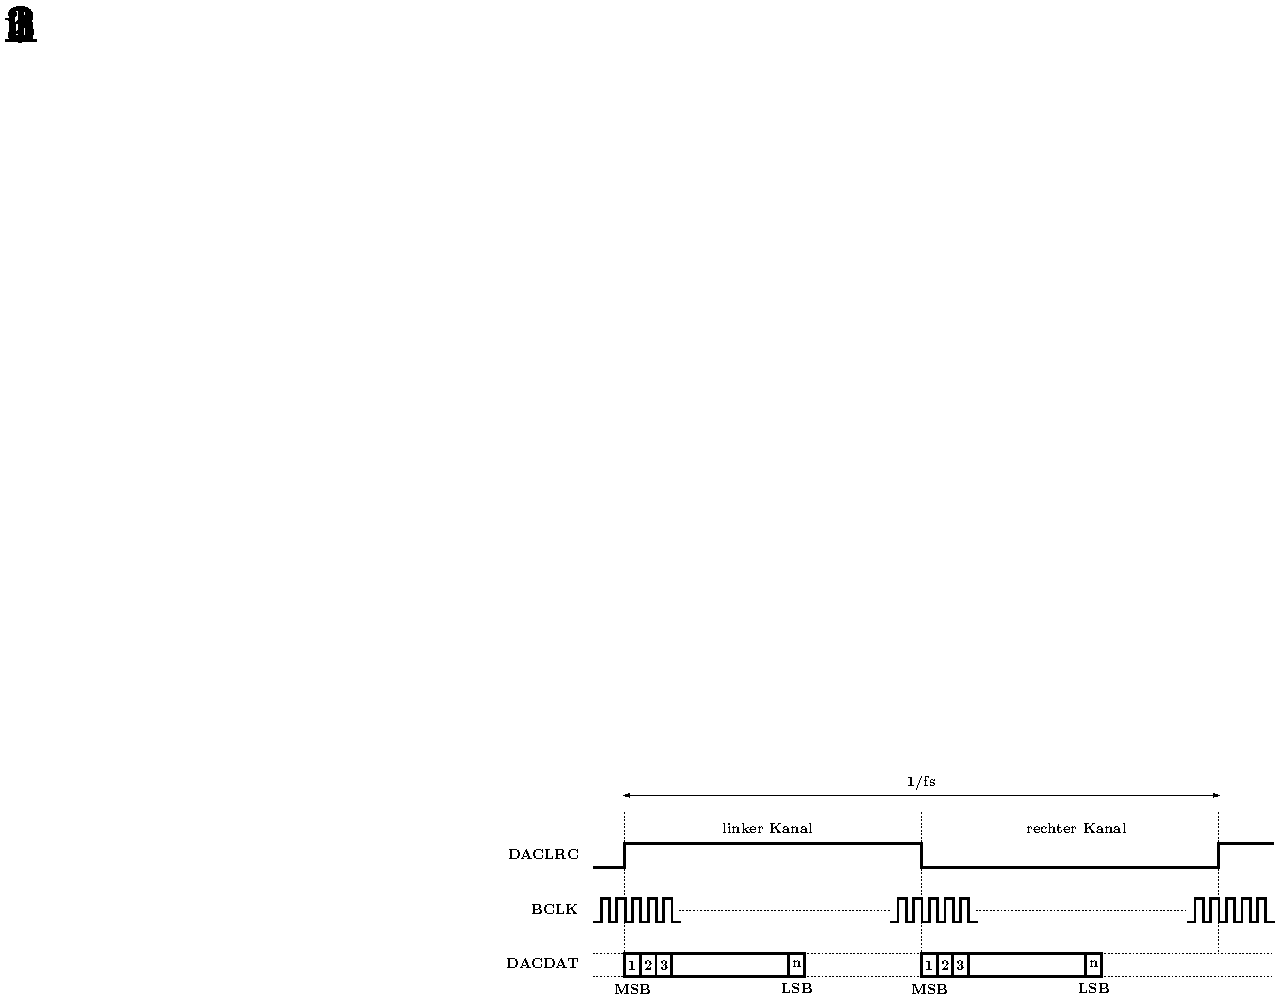
\includegraphics[width=1\textwidth]{Codec_Signals_Serializer.pdf}
	\caption{Signalverlauf des Codec Interface} 
	\label{img:Codec_Signals}
\end{figure}  